\documentclass[a4paper,14pt]{extarticle}

\usepackage[utf8x]{inputenc}
\usepackage[T1,T2A]{fontenc}
\usepackage[russian]{babel}
\usepackage{hyperref}
\usepackage{indentfirst}
\usepackage{here}
\usepackage{array}
\usepackage{graphicx}
\usepackage{caption}
\usepackage{subcaption}
\usepackage{chngcntr}
\usepackage{amsmath}
\usepackage{amssymb}
\usepackage{pgfplots}
\usepackage{pgfplotstable}
\usepackage[left=2cm,right=2cm,top=2cm,bottom=2cm,bindingoffset=0cm]{geometry}
\usepackage{multicol}

\renewcommand{\le}{\ensuremath{\leqslant}}
\renewcommand{\leq}{\ensuremath{\leqslant}}
\renewcommand{\ge}{\ensuremath{\geqslant}}
\renewcommand{\geq}{\ensuremath{\geqslant}}
\renewcommand{\epsilon}{\ensuremath{\varepsilon}}
\renewcommand{\phi}{\ensuremath{\varphi}}

\counterwithin{figure}{section}
\counterwithin{equation}{section}
\counterwithin{table}{section}
\newcommand{\sign}[1][5cm]{\makebox[#1]{\hrulefill}} % Поля подписи и даты
\graphicspath{{pics/}} % Путь до папки с картинками
\captionsetup{justification=centering,margin=1cm}
\def\arraystretch{1.3}

\begin{document}

\begin{titlepage}
\begin{center}
	\textbf{Санкт-Петербургский Политехнический Университет \\Петра Великого}\\[0.3cm]
	\small Институт компьютерных наук и технологий \\[0.3cm]
	\small Кафедра компьютерных систем и программных технологий\\[4cm]
	
	\textbf{ОТЧЕТ}\\ \textbf{о лабораторной работе}\\[0.5cm]
	\textbf{<<Исследование частотных характеристик пассивных RC-цепей>>}\\[0.1cm]
	\textbf{Электротехника и Электроника}\\[10.5cm]
\end{center}

\begin{flushright}
	\begin{minipage}{0.60\textwidth}
		\begin{flushleft}
			\small \textbf{Работу выполнили студенты}\\[3mm]
			\small группа 23501/4 \hspace*{17mm} Дьячков В.В.\\[3mm]
			\small группа 23501/4 \hspace*{17mm} Ламтев А.Ю.\\[5mm]
			
			\small \textbf{Преподаватель}\\[5mm]
		 	\small \sign[3.5cm] \hspace*{8mm} к.т.н., доц. Кочетков Ю.Д.\\[0.5cm]
		\end{flushleft}
	\end{minipage}
\end{flushright}

\vfill

\begin{center}
	\small Санкт-Петербург\\
	\small \the\year
\end{center}
\end{titlepage}

\section{Цель работы}

Исследование RC-генераторов синусоидальных колебаний с постоянной и управляемой частотой, их настройка, сравнение теоретических и экспериментальных результатов.

\section{Чертеж схемы исследуемого устройства}

\begin{figure}[H]
\begin{center}
	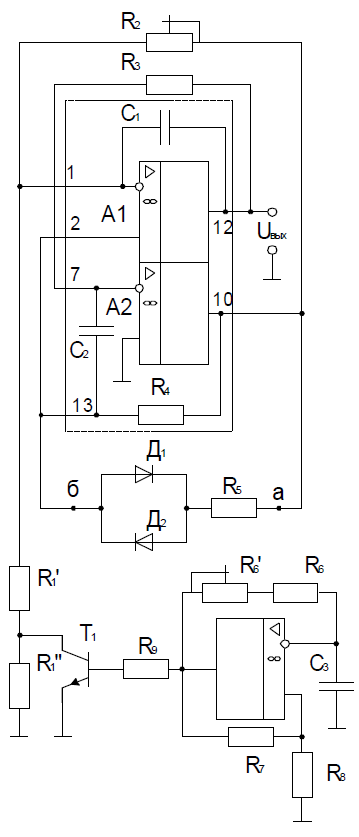
\includegraphics[width=0.45\textwidth]{scheme}
	\caption{Схема управляемого генератора}
\end{center}
\end{figure}

\section{Исходные данные}

\begin{table}[H]
\begin{center}
	\caption{Исходные данные}
	\def\tabcolsep{8pt}
	\begin{tabular}{|c|c|c|c|c|c|c|c|c|c|c|c|c|}
		\hline
		$E{01}$, В &
		$E{02}$, В &
		$f_0$, кГц &
		$R_3$, кОм &
		$R_4$, кОм &
		$R_5$, кОм &
		$R_6$, кОм \\
		\hline
		15 &
		-15 &
		65 &
		33 &
		6.8 &
		24 &
		8.2 \\
	    \hline	
	\end{tabular}
\end{center}
\end{table}

\begin{table}[H]
\begin{center}
	\def\tabcolsep{8pt}
	\begin{tabular}{|c|c|c|c|c|c|c|c|c|c|c|c|c|}
		\hline
		$R_6^*$, кОм &
		$R_7$, кОм &
		$R_8$, кОм &
		$R_9$, кОм &
		$C_1$, нФ &
		$C_2$, нФ \\
		\hline
		1 &
		8.2 &
		3.9 &
		1.3 &
		1 &
		2 \\
	    \hline	
	\end{tabular}
\end{center}
\end{table}

\section{Теоретические расчёты}

\begin{equation}
\label{eq:4:1}
	R_\text{2 min} = \frac{R_4 \cdot C_2}{C_1} = \frac{6.8 \cdot 10^3 \cdot 2 \cdot 10^{-9}}{10^{-9}} = 13.6 \text{ кОм}
\end{equation}

\begin{equation}
	R_1 = \left((2\pi f_0)^2 R_3 C_1 C_2 \right)^{-1} = \left((2\pi \cdot 6.5 \cdot 10^3)^2 \cdot 33 \cdot 10^3 \cdot 2 \cdot 10^{-9} \cdot 10^{-9} \right)^{-1} = 9 \text{ кОм}
\end{equation}

\begin{equation}
	C_3 = \frac{16}{f_0 \cdot R_6} = \frac{16}{6.5 \cdot 10^3 \cdot 8.2 \cdot 10^3} = 300 \text{ нФ}
\end{equation}

\begin{equation}
	f_1 = f_0 \cdot \sqrt{\frac{2}{5}} = 4.11 \text{ кГц}
\end{equation}

\begin{equation}
\label{eq:4:5}
	f_2 = f_0 \cdot \sqrt{2} = 9.19 \text{ кГц}
\end{equation}

\section{Экспериментально снятые зависимости}

\subsection{Генератор гармонических колебаний без задающего мультивибратора и транзисторного ключа}

\begin{displaymath}
	f = 6.21 \text{ кГц}
\end{displaymath}

\begin{displaymath}
	R_2 = 15.43 \text{ кОм}
\end{displaymath}


\begin{table}[H]
\begin{center}
	\caption{Зависимость $f_0 = f(R_1)$}
	\label{tab:diff-int}
	\def\tabcolsep{20pt}
	\pgfplotstabletypeset[col sep=comma,
	    columns={r,f0},
	    column type/.add={|c|}{},
	    columns/r/.style={fixed, column name={$R_1$, кОм}},
	    columns/f0/.style={fixed, precision=3, zerofill, column name={$f_0$, кГц}},
	    every nth row={1}{before row=\hline},
	    every head row/.style={before row=\hline, after row=\hline},
	    every last row/.style={after row=\hline}
	   ]{data/f0_as_f_of_R_exp.csv}
\end{center}
\end{table}

\begin{figure}[H]
\begin{center}
	\begin{tikzpicture} [every plot/.append style={thick}]
		\begin{axis}[
			height=0.45\textheight,
			width=0.95\textwidth,
			legend pos = north east,
			xlabel={$R_1$, кОм},
			ylabel={$f_0$, кГц},
			axis x line = middle,
			axis y line = left,
			xmode=linear,
			xmin = 0,
			xmax = 130,
			ymin = 0,
			ymax = 14,
			grid=major
		]
		\addplot [smooth, mark=square*, blue] table[x=r,y=f0,col sep=comma]{data/f0_as_f_of_R_exp.csv};
		\addplot [smooth, red] table[x=r,y=f0,col sep=comma]{data/f0_as_f_of_R_theory.csv};
		\legend{Эксп., Теор.}
		\end{axis}
	\end{tikzpicture}
	\caption{Зависимость $f_0 = f(R_1)$}
	\label{plot:rectifier}
\end{center}
\end{figure}

\subsection{Генератор гармонических колебаний c подключенными задающим мультивибратором и транзисторным ключом}

\begin{displaymath}
	R_2 = 16.32 \text{ кОм}
\end{displaymath}

\begin{displaymath}
	U_\text{ампл}^\text{лин} = 2.78 \text{ В}
\end{displaymath}

\begin{displaymath}
	U_\text{ампл}^\text{нелин} = 2.6 \text{ В}
\end{displaymath}

\begin{displaymath}
	R_1^{'} = \frac{R_1}{2} = \frac{9 \cdot 10^3}{2 \cdot 10^3} = 4.5 \text{ кОм}
\end{displaymath}

\begin{displaymath}
	R_1^{''} = 2 \cdot R_1 = 9 \cdot 10^3 \cdot 2 = 18 \text{ кОм}
\end{displaymath}

\begin{figure}[H]
\begin{tikzpicture}
\begin{axis} [
	ticks=none,
	width=\textwidth,
	height=6cm,
	grid=both,
	minor tick num=1,
	axis x line=center, 
	axis y line=left, 
	xlabel=$t$,
	ymin=-20,
	ymax=20,
%	xmin=-200,
%	xmax=200,
	ylabel=$U_\text{вых}(t)$
] 
\addplot [black, thick, mark=none] coordinates {(0, 14) (2, 14)};
\addplot [black, thick, mark=none] coordinates {(2, 14) (2, -14)};
\addplot [black, thick, mark=none] coordinates {(2, -14) (7, -14)};
\addplot [black, thick, mark=none] coordinates {(7, -14) (7, 14)};
\addplot [black, thick, mark=none] coordinates {(7, 14) (12, 14)};
\addplot [black, thick, mark=none] coordinates {(12, 14) (12, -14)};
\addplot [black, thick, mark=none] coordinates {(12, -14) (14, -14)};
\addplot [black, domain=0:2, samples=200] {sin(x*1200 + 90) * 13 * (1 - x / 25)};
\addplot [black, domain=2:7, samples=200] {sin(x*700) * 10 * (1 - (x ) / 25)};
\addplot [black, domain=7:12, samples=200] {sin(x*1000 + 50) * 13  * (1 - (x - 7) / 25)};
\addplot [black, domain=12:14, samples=200] {sin(x*500 - 70) * 10 * (1 - (x - 7) / 25) };
\end{axis}
\end{tikzpicture}
\caption{Выходной сигнал генератора колебаний}
\label{osc}
\end{figure}

\begin{displaymath}
	f_1 = 4.17 \text{ кГц}
\end{displaymath}

\begin{displaymath}
	f_2 = 9.28 \text{ кГц}
\end{displaymath}

\section{Погрешности}

\subsection{Предельно допустимые порешности}

\begin{displaymath}
\delta_{max} f = \sqrt{\left(\frac{1}{2} \cdot \delta R_1 \right)^2 + \left(\frac{1}{2} \cdot \delta R_3 \right)^2} = \sqrt{\left(\frac{1}{2} \cdot 0.1 \right)^2 + \left(\frac{1}{2} \cdot 0.1 \right)^2} = 0.071 = 7.1\%
\end{displaymath}

\subsection{Приведённые погрешности}

\begin{displaymath}
	\delta f_1 = \left|\frac{f_\text{1 теор.} - f_\text{1 эксп.}}{f_\text{1 теор.}} \right| = \left|\frac{4.11 \cdot 10^3 - 4.17 \cdot 10^3}{4.11 \cdot 10^3}\right| = 0.015 = 1.5\% < \delta_{max} f = 7.1\%
\end{displaymath}

\begin{displaymath}
	\delta f_2 = \left|\frac{f_\text{2 теор.} - f_\text{2 эксп.}}{f_\text{2 теор.}} \right| = \left|\frac{9.19 \cdot 10^3 - 9.28 \cdot 10^3}{9.19 \cdot 10^3}\right| = 0.01 = 1\% < \delta_{max} f = 7.1\%
\end{displaymath}

\section{Выводы}

Приведённые погрешности полученных в ходе эксперимента значений $f$ не превышают предельно допустимые погрешности.

Таким образом, формулы \ref{eq:4:1} -- \ref{eq:4:5} являются верными.

\end{document}